%!TEX root = ../thesis.tex
%*******************************************************************************
%****************************** Third Chapter **********************************
%*******************************************************************************
\chapter{Design}
\graphicspath{{Chapter5/Figs/Raster/}{Chapter5/Figs/Tex/}{Chapter5/Figs/}}

Following the discussion in Chapter 2.3.1 and 2.5, the designs for this project 
will be created on top of Hyperledger Fabric, a public permissioned blockchain.
It has become clear that a blockchain specific, high-fidelity prototyping tool is needed 
to create system designs such as data and transaction models.

\section{Design Tool}

Hyperledger Composer is an open source development toolset and framework that aims to 
accelerate time to value for blockchain projects. It offers business-centric 
abstractions, allowing business owners and developers to rapidly develop 
use cases and model a blockchain network. The design tools offered take the forms of:
\begin{itemize}
    \setlength\itemsep{0em}            
    \item An object-oriented modelling language (.cto file) to define data models in 
    the blockchain network
    \item JavaScript functions (.js file) to define logic for smart contracts triggered by transactions
    \item An access control language (.acl file) to define access rules for records on the blockchain\\
    \citep{official2018composer}
\end{itemize}

See Figure \ref{fig:composer2fabric} for a visual explainer of how Hyperledger Composer 
helps designers and developers create these high level definitions.

\begin{figure}[!ht] 
    \centering    
    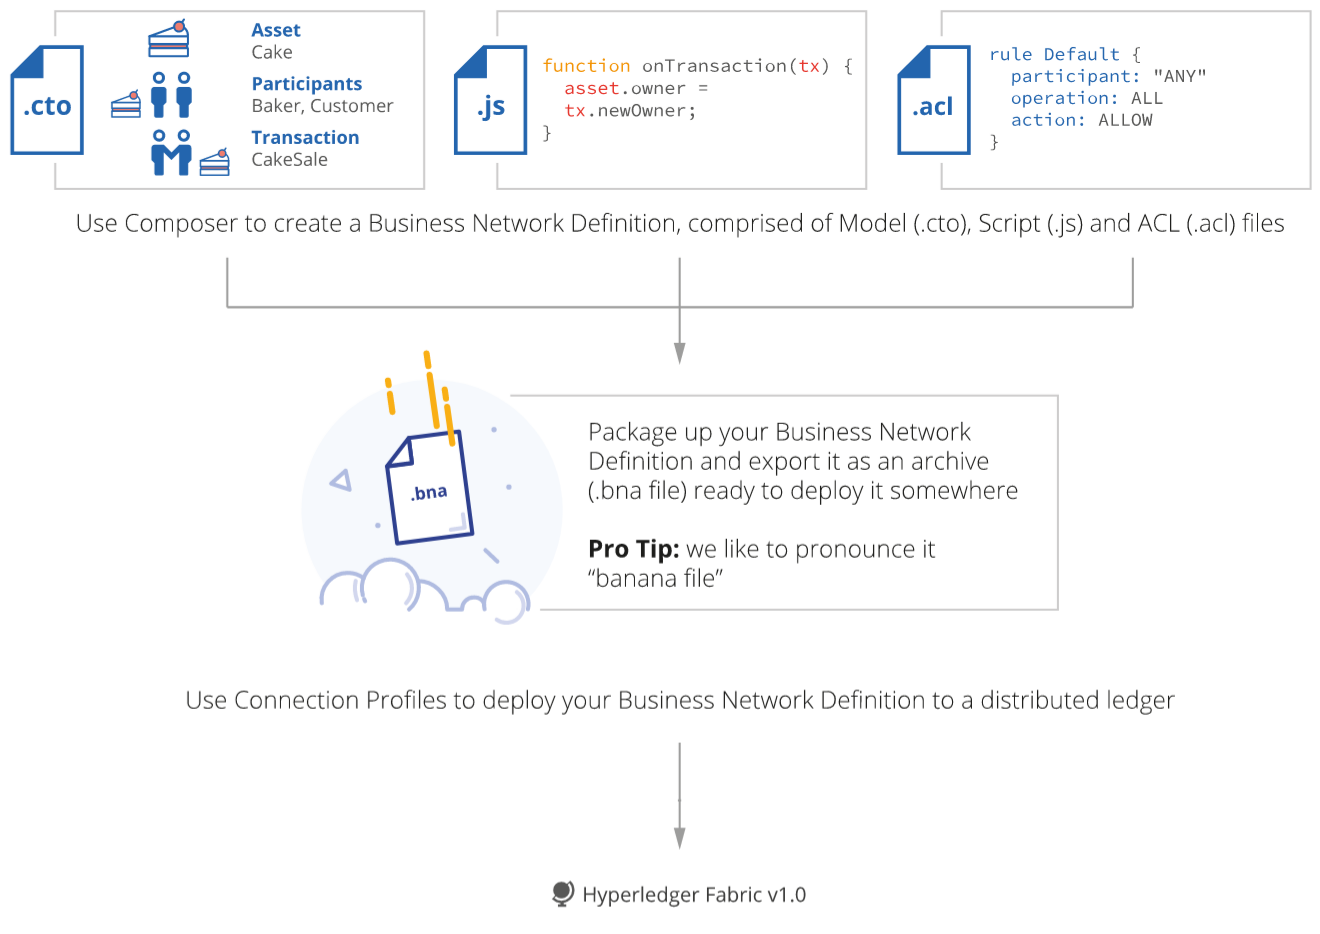
\includegraphics[width=1.0\textwidth]{composer2fabric}
    \caption[Hyperledger Composer]
        {Components in the Hyperledger Composer framework and how it deploys to 
        Hyperledger Fabric \citep{cuicapuza2017composer}} 
    \label{fig:composer2fabric}
\end{figure}
% https://medium.com/@RichardCuica/hyperledgers-fabric-composer-simplifying-business-networks-on-blockchain-94313b979671

A significant advantage of using Hyperledger Composer is its ability to package these 
prototype definitions and deploy it to Hyperledger Fabric, our target blockchain platform. 
This will speed up the implementation of the proposed demonstrator applications 
in the next stage.

Throughout the design process, the Hyperledger Composer notations are converted into UML sequence 
diagrams, class diagrams and activity diagrams with PlantUML, an open source language-to-diagram drawing tool.

The discussion below may regularly refer back to the functional requirements (FR) and 
non-functional requirements (NR) defined in the previous Chapter 4.

\section{Transaction Sequences}

A transaction is the only activity that a peer can perform to alter the state of the blockchain. 
Designing the sequences of transactions necessary to fulfil the desired use journeys will  
be able to provide a good overview of the work ahead, and the fields that data model 
objects should include to enable these transactions. Two overarching use cases are considered: 
assessment and curriculum personalisation.

\subsection{Assessment Use Case}

These four transactions are required to complete the assessment use case (see Figure \ref{fig:assessmentloop}):

\begin{figure}[!ht] 
    \centering    
    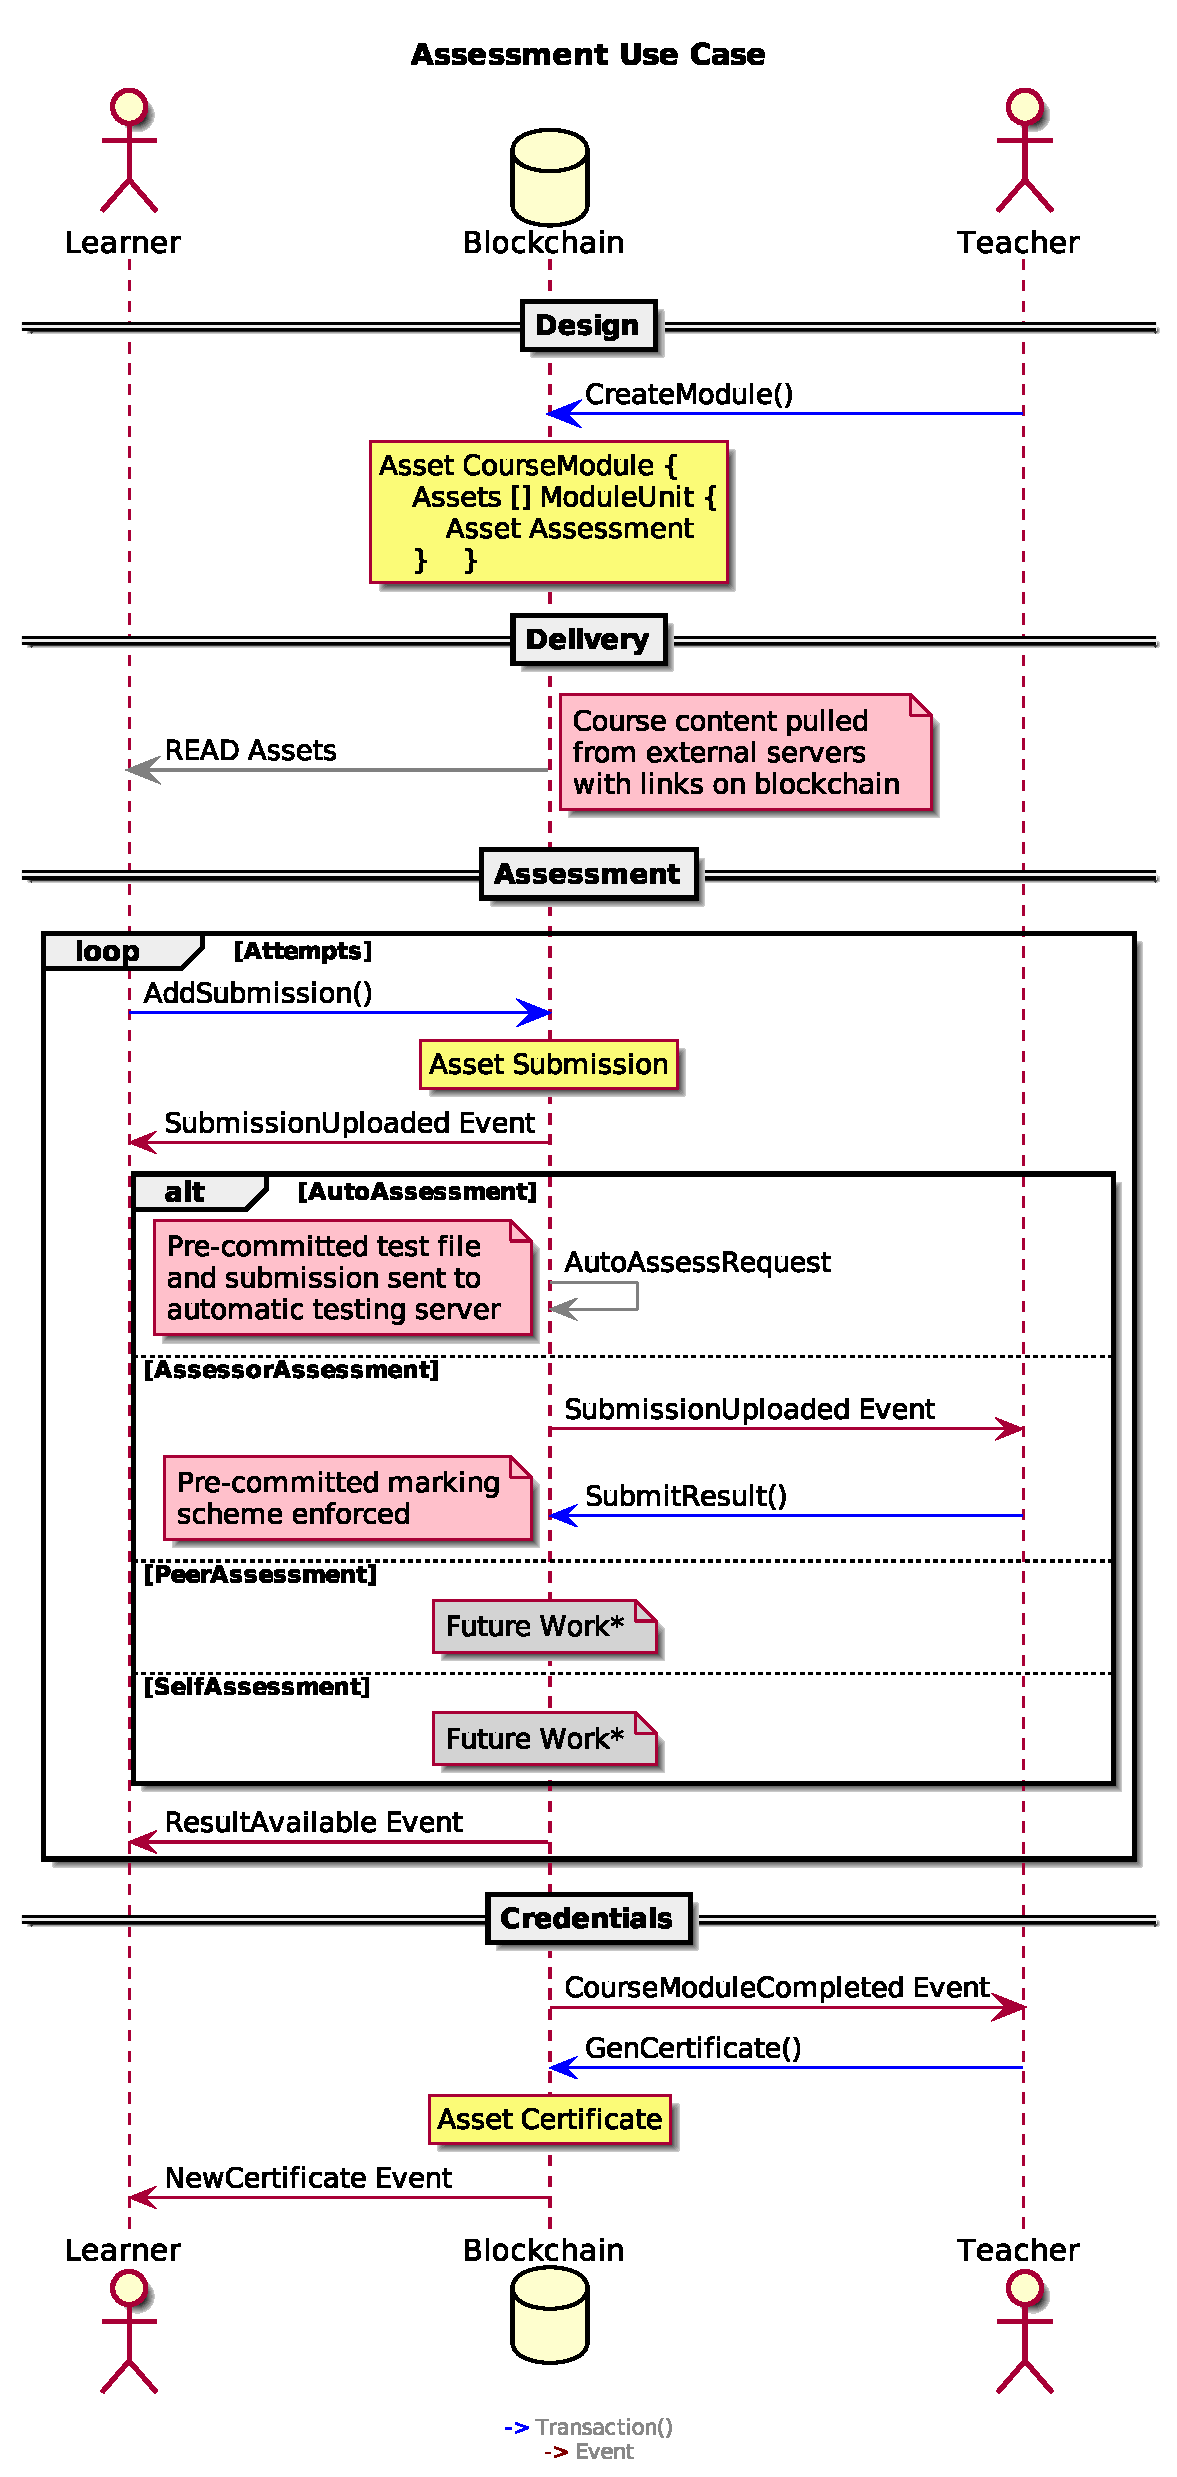
\includegraphics[width=0.65\textwidth]{assessmentloop}
    \caption[Assessment Use Case]
        {A UML sequence diagram denoting the assets, transactions and events between 
        learner and teacher participants on the blockchain for the assessment use case} 
    \label{fig:assessmentloop}
\end{figure}

\begin{itemize}
    \setlength\itemsep{0em}        
    \item CreateModule: a transaction ordered by a teacher to store metadata about a course module, 
    its units and assessments onto the blockchain;
    \item AddSubmission: a transaction ordered by a learner to store a submission (assessment attempt) 
    on the blockchain, this could return the result of the assessment if the result is returned by 
    an automatic (machine) marking service;
    \item SubmitResult: a transaction ordered by a teacher to store details of an assessor assessment 
    on the blockchain;
    \item GenCertificate: a transaction ordered by a teacher to create a new certificate on the blockchain.
\end{itemize}

\subsection{Curriculum Personalisation Use Case}

Similarly, we looked at the transactions required to build a minimum viable product 
that facilitates curriculum personalisation. A curriculum here is simply a list of course 
modules attached to a learner and a teacher (a personal tutor for the learner).

\begin{itemize}
    \setlength\itemsep{0em}            
    \item ProposeCurriculum: a transaction ordered by a learner or a teacher to propose 
    a brand new curriculum, or to proposed edits to an existing curriculum on the blockchain.
    \item ApproveCurriculum: a transaction ordered by a teacher to enrol a learner to 
    the course modules in the learner's curriculum.
\end{itemize}

See Figure \ref{fig:personalisationloop} for where these two transactions occur in a sequence diagram.

\begin{figure}[!ht] 
    \centering    
    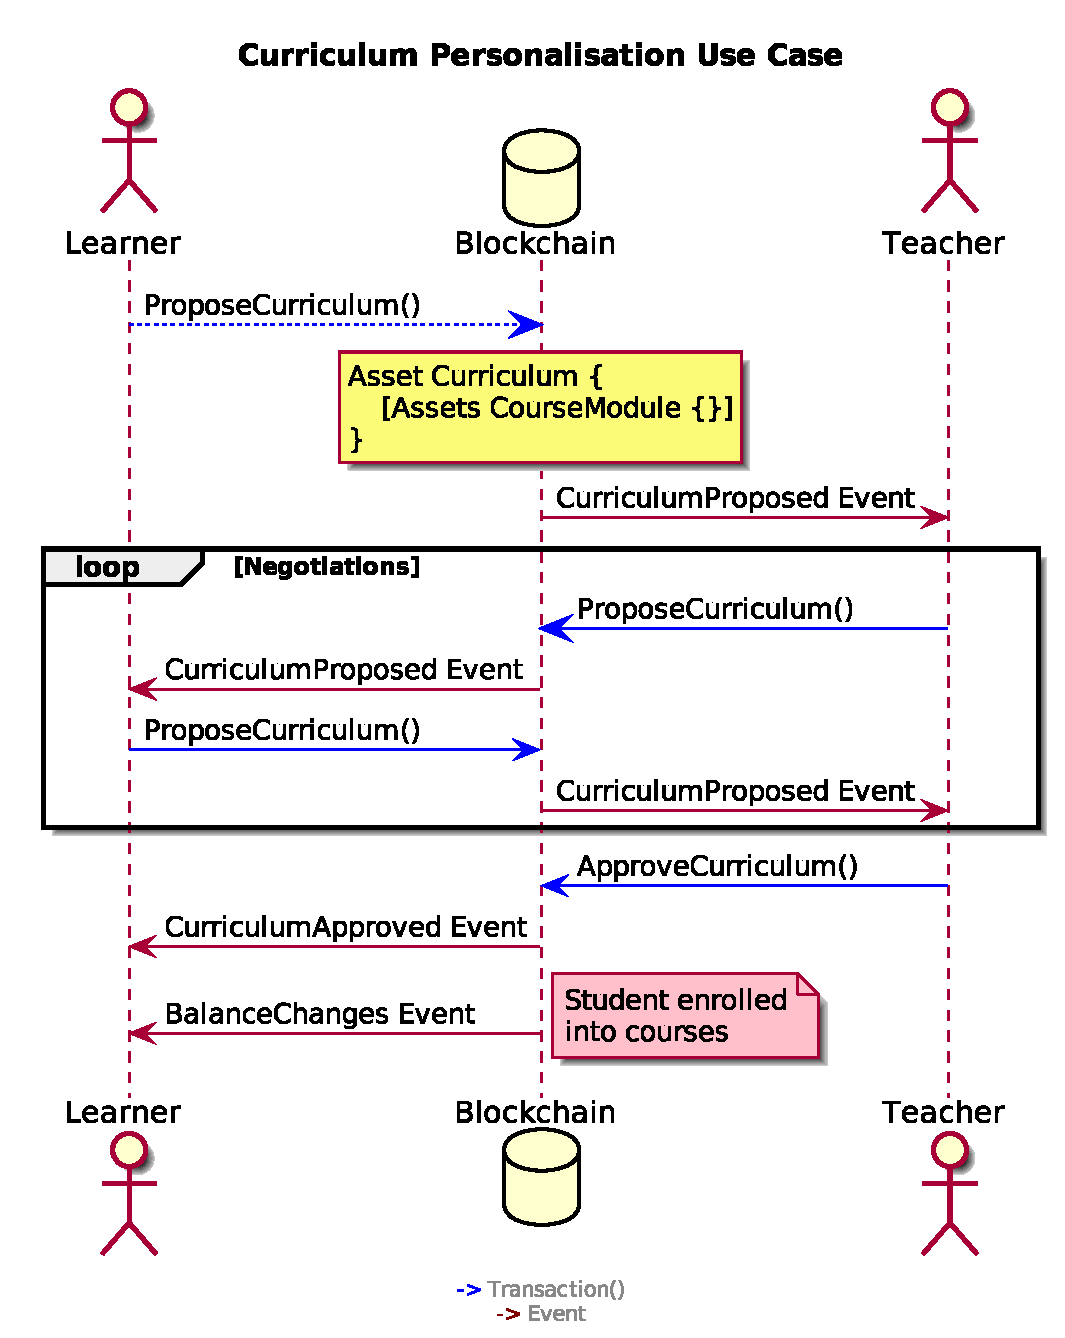
\includegraphics[width=0.7\textwidth]{personalisationloop}
    \caption[Curriculum Personalisation Use Case]
        {Sequence diagram denoting the assets, transactions and events between 
         learner and teacher participants on the blockchain for the curriculum personalisation use case} 
    \label{fig:personalisationloop}
\end{figure}

% automatic formative assessments Annette's student

% schema --> reviewer

\section{Data Models}

Building a blockchain network requires a network-wide schema of what records are allowed to be created, updated and read. 
The Hyperledger Composer framework calls these resource definitions, and recommends defining objects 
inheriting three basic types: Participants, Assets and Concepts in its object-oriented modelling language 
\citep{official2018composer}.

\subsection{Participants}

A participant is an actor in a blockchain network. A participant can create and exchange other assets 
by submitting transactions \citep{official2018composer}.
The network design for this project will allow the creation of three main types of participants: 
\begin{itemize}
    \setlength\itemsep{0em}    
    \item \textit{Teacher}, which can be lecturers, teaching assistants, tutors, etc.
    \item \textit{Learner}, which can be campus students, distant learners, etc.
    \item \textit{Reader}, members of the public who are interested in querying or verifying records, 
    such as employers and further education providers.
\end{itemize}

All three types of participants inherit an abstract (cannot be created) class \textit{User}. The \textit{nid} field 
that all \textit{Users} must have would contain a one-way hash of their national identification number, which can be a 
driver's license number, social security number, etc. A hash is a form 
of cryptographical representation of data that is non-invertible. This allows the system to ensure that 
all writers in the system is known and unique, while protecting their privacy to the general public.

See Figure \ref{fig:participants} for the detailed entity properties of all participant types 
in a class diagram.

\begin{figure}[!ht] 
    \centering    
    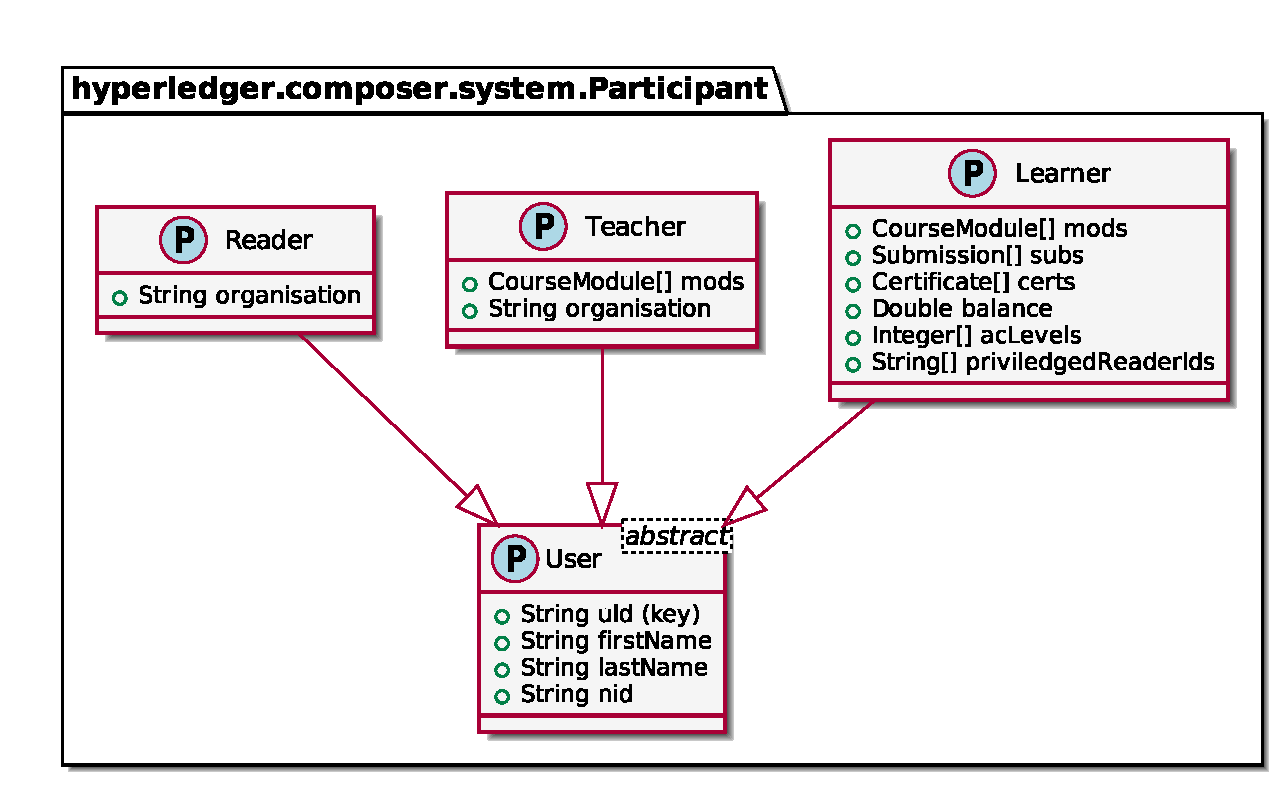
\includegraphics[width=0.7\textwidth]{participants}
    \caption[Participants Class Diagram]
        {A UML class diagram describing the participants defined on the blockchain} 
    \label{fig:participants}
\end{figure}

A notable design consideration is the mechanism for allowing tiered access control of 
learner information. The \textit{acLevels} and \textit{priviledgedReaderIds} fields in \textit{Learner}
store access control settings for two tiers of \textit{Readers}, normal and privileged. 
This will be covered in more detail in an upcoming section.

\subsection{Assets}

Assets are "tangible or intangible goods, services, or property, and are stored in registries" \citep{official2018composer}.
The asset definitions are modelled carefully according to literature and user requirements.
See Figure \ref{fig:assets} for the detailed entity properties and relationships of these assets 
in a class diagram.

\begin{figure}[!ht] 
    \centering    
    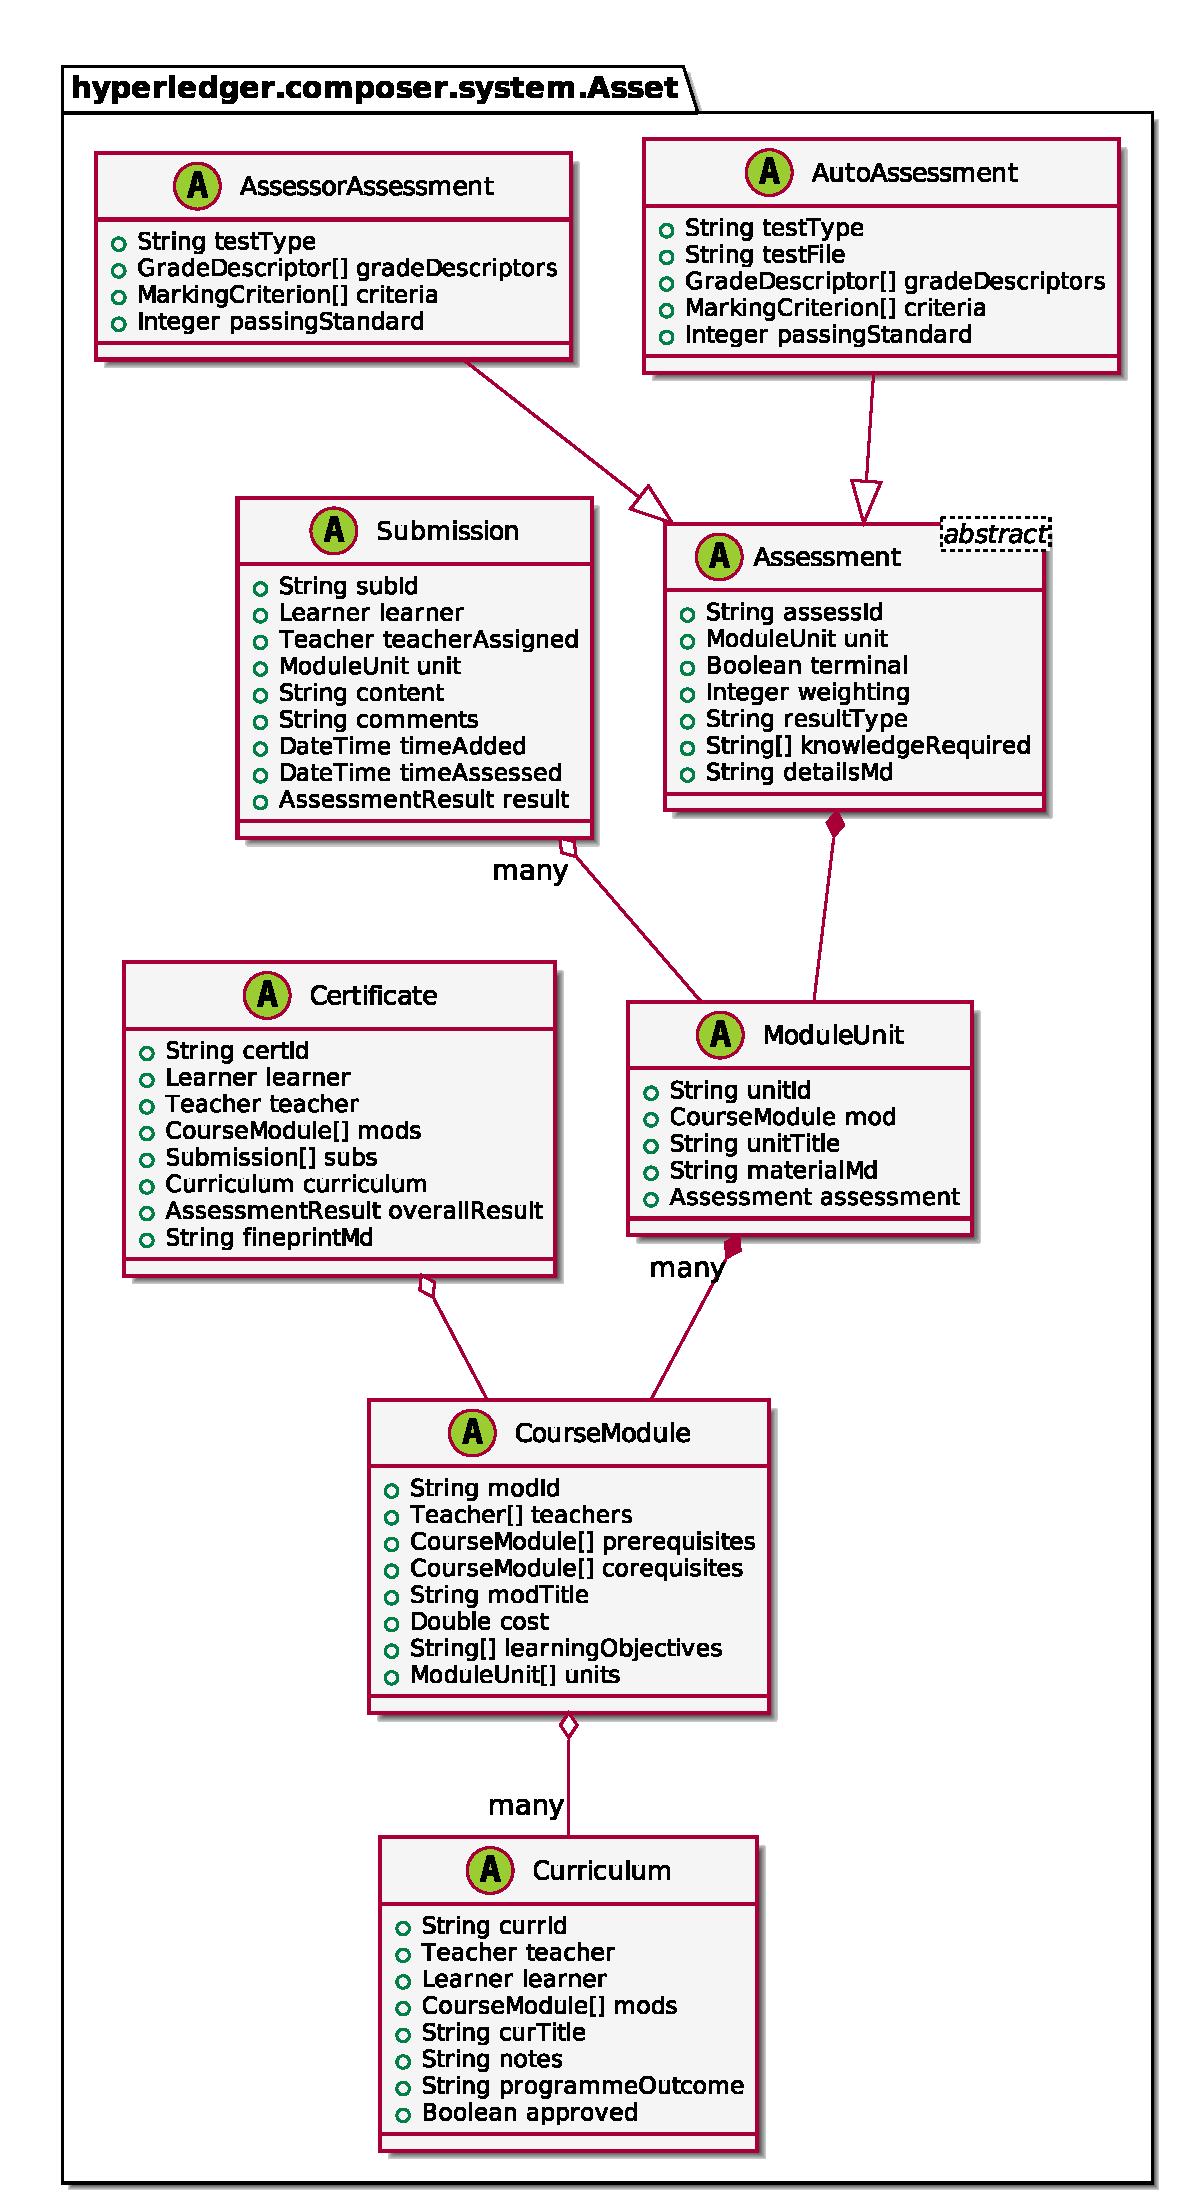
\includegraphics[width=0.65\textwidth]{assets}
    \caption[Assets Class Diagram]
        {A UML class diagram describing the assets defined on the blockchain} 
    \label{fig:assets}
\end{figure}

The special design considerations included:
\begin{itemize}
    \setlength\itemsep{0em}            
    \item Types of assessments: Online assessments may be grouped in four categories (TODO: Paulsen, 2003, page 68): 
    self-assessment, computer assessment, tutor assessment, and peer assessment. Why two in future work?
    \item knowledge required, learning objective
    \item programme outcomes: middleman fields bureaucracy
    \item Markdown fields: Markdown is [TODO]. It is anticipated that many markets, institutions, departments and teachers 
    will have their own requirements, format and templates for what their e-Learning content should look like. To cater to 
    this need for content and layout flexibility the blockchain will accept markdown syntax as input in fields such as 
    detailsMd in Assessment, materialMd in ModuleUnit and fineprintMd in Certificate.
    \item Assessments: grade descriptors and criteria
\end{itemize}

\subsection{Concepts}

Concepts are abstract classes that are not assets or participants. They are used to define custom properties contained by an asset or participant.

\begin{figure}[!ht] 
    \centering    
    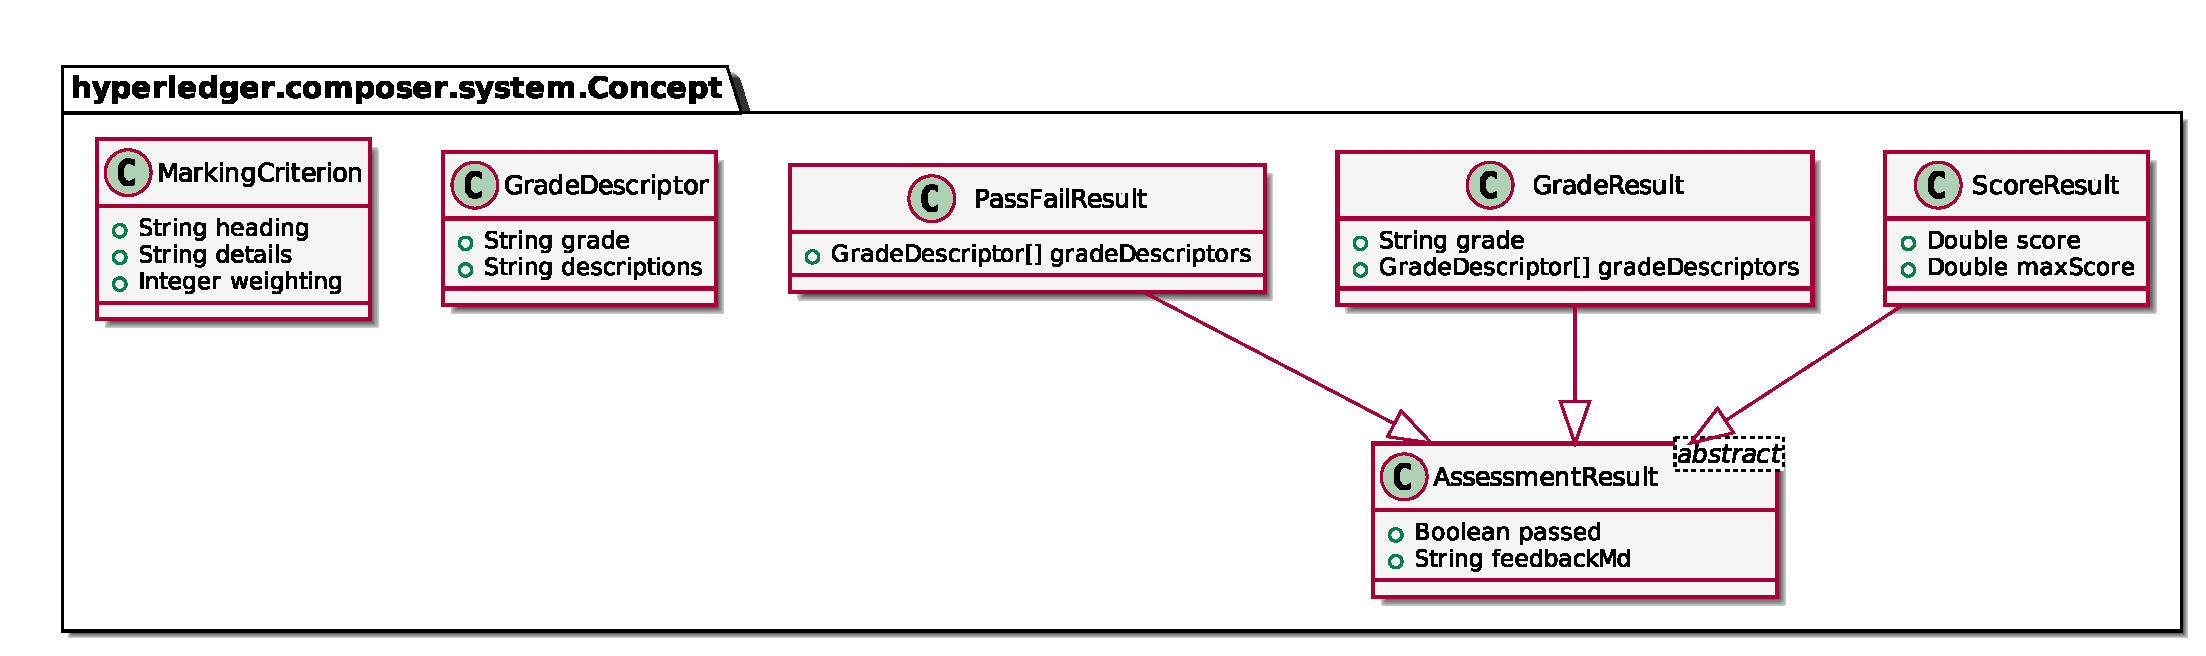
\includegraphics[width=1.0\textwidth]{concepts}
    \caption[Concepts Class Diagram]
        {A UML class diagram describing the concepts (other abstract classes that are contained as a field) defined on the blockchain} 
    \label{fig:concepts}
\end{figure}

\section{Smart Contracts: Transaction Logic and Events}

We have previously discussed the nature of Smart Contracts in Chapter 2.3.2. They are autonomous, self-sufficient and 
decentralised code that runs on a blockchain. In Hyperledger Composer, Smart Contracts are called chaincode and 
they are run synchronously with a transaction order, with a final output required to accept the transaction or reject it.

\subsection{The CreateModule Transaction}
\begin{figure}[!ht]
    \centering
    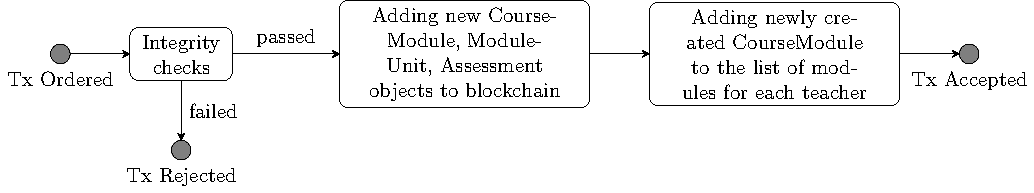
\includegraphics[width=1.0\textwidth]{cmtx}
    \caption{A flowchart representation of the Smart Contract behind the CreateModule Transaction (Tx)} \label{fig:cmtx}
\end{figure}

\subsection{The AddSubmission Transaction}

\begin{figure}[!ht]
    \centering
    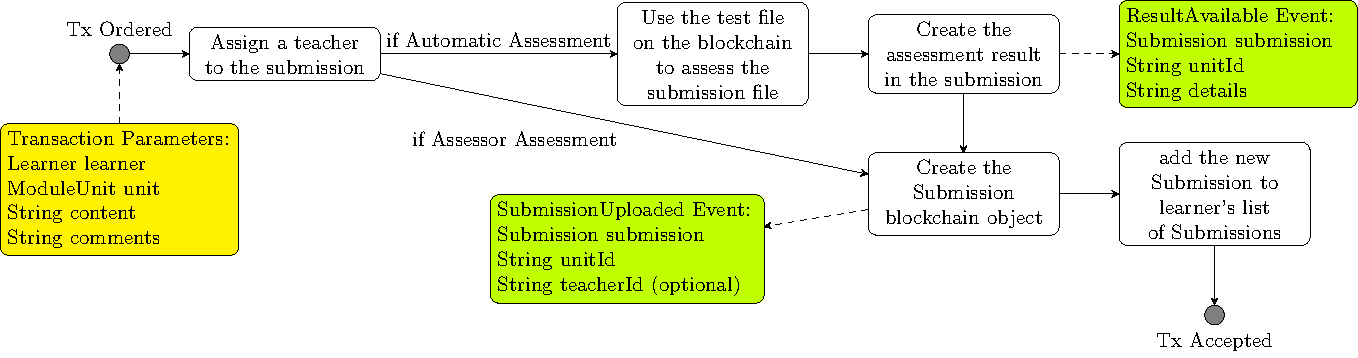
\includegraphics[width=1.0\textwidth]{astx}
    \caption{A flowchart representation of the Smart Contract behind the AddSubmission Transaction (Tx)} \label{fig:astx}
\end{figure}

\subsection{The SubmitResult Transaction}

\subsection{The GenCertificate Transaction}

\subsection{The ProposeCurriculum Transaction}

\subsection{The ApproveCurriculum Transaction}


\section{Access Control}
Role based and attribute based

\section{Limitations}
No institutional approvers for certificates
No different tiers of privileges for teachers for roles such as module leader, module reviewer, supporting staff

\section{User Interfaces for Client Applications}

While improving general usability is not one of the objectives of this project, poor usability and interface designs 
could negate the improvements in assessments and curriculum personalisation that this project aims for.

Adopt a popular design language for the user interfaces in the client applications.

Paper prototypes that follow usability hieuristics.